% Capital Allocation I -- how much risk, and whose. The frontier, the formula, and how your job and your mandate tilt it.
% Figures and every number quoted here come from capital_allocation_figures.py
% Companion notebook: chapters/Finance/L12_CapitalAllocationI_v2_AI.ipynb (sections 1-6 in class, the challenge is homework)
% The challenge answers (the 49 industries) must not appear here: this PDF is public.
% The mechanics use the six factors. The tilts and the mandates use the eight sectors, because they need sectors with names.
\documentclass[aspectratio=169,10pt]{beamer}
\usetheme{default}
\usecolortheme{default}

\usepackage{graphicx}
\usepackage{adjustbox}
\usepackage{amsmath}
\usepackage{amssymb}
\usepackage{booktabs}
\usepackage{array}
\usepackage{tikz}
\usetikzlibrary{arrows.meta,positioning,calc,decorations.pathreplacing}
\usepackage{appendixnumberbeamer}  % Exclude appendix from slide count

\setbeamertemplate{navigation symbols}{}
\setbeamertemplate{items}[circle]

% Footline: Author, Event (Year) on left; page/total on right
\setbeamertemplate{footline}{
  \hbox{%
    \begin{beamercolorbox}[wd=.5\paperwidth,ht=2.5ex,dp=1ex,left]{author in head/foot}%
      \hspace*{2ex}\insertshortauthor, \insertshortinstitute\ (\insertdate)
    \end{beamercolorbox}%
    \begin{beamercolorbox}[wd=.5\paperwidth,ht=2.5ex,dp=1ex,right]{date in head/foot}%
      \insertframenumber/\inserttotalframenumber\hspace*{2ex}
    \end{beamercolorbox}%
  }
}

% Highlight boxes
\setbeamercolor{box1}{bg=red!12,fg=black}

% A poll option: {colour}{letter and choice}
\newcommand{\pollbox}[2]{\tikz\node[draw=#1!65!black, fill=#1!10, rounded corners=4pt, minimum width=3.7cm,
                                   minimum height=1.0cm, align=center, font=\normalsize]{#2};}
\newcolumntype{P}[1]{>{\raggedright\arraybackslash}p{#1}}

\title{Capital Allocation I}
\subtitle{How much risk, and whose}
\author[A. Moreira]{Alan Moreira}
\institute[Data-Driven Investing]{NYU Stern --- Data-Driven Investing}
\date{Fall 2026}

\begin{document}

\begin{frame}
\titlepage
\end{frame}

\begin{frame}{Today}
\vskip 6pt
\begin{columns}[t]
\begin{column}{0.46\textwidth}
\textbf{In the slides}
\vskip 6pt
\begin{itemize}
\item The frontier, and the formula behind it
\vskip 6pt
\item When a new asset moves the frontier: the alpha test
\vskip 6pt
\item How your job and your mandate tilt the portfolio
\end{itemize}
\end{column}
\begin{column}{0.50\textwidth}
\textbf{In the notebook, you will}
\vskip 6pt
\begin{itemize}
\item Build the tangency and minimum-variance portfolios on six factors, step by step
\vskip 6pt
\item Draw the frontier from those two
\vskip 6pt
\item Size one portfolio for different goals
\vskip 6pt
\item Run the alpha test on momentum and on HML
\end{itemize}
\end{column}
\end{columns}
\vskip 16pt
\begin{beamercolorbox}[rounded=true,sep=7pt,center]{box1}
\textbf{Homework:} goals and mandates on the 49 industries
\end{beamercolorbox}
\end{frame}

%================================================================== THE PICTURE
\begin{frame}{Everyone wants to be on the line}
\begin{columns}[c]
\begin{column}{0.62\textwidth}
\adjustbox{max width=\textwidth, max height=0.74\textheight}{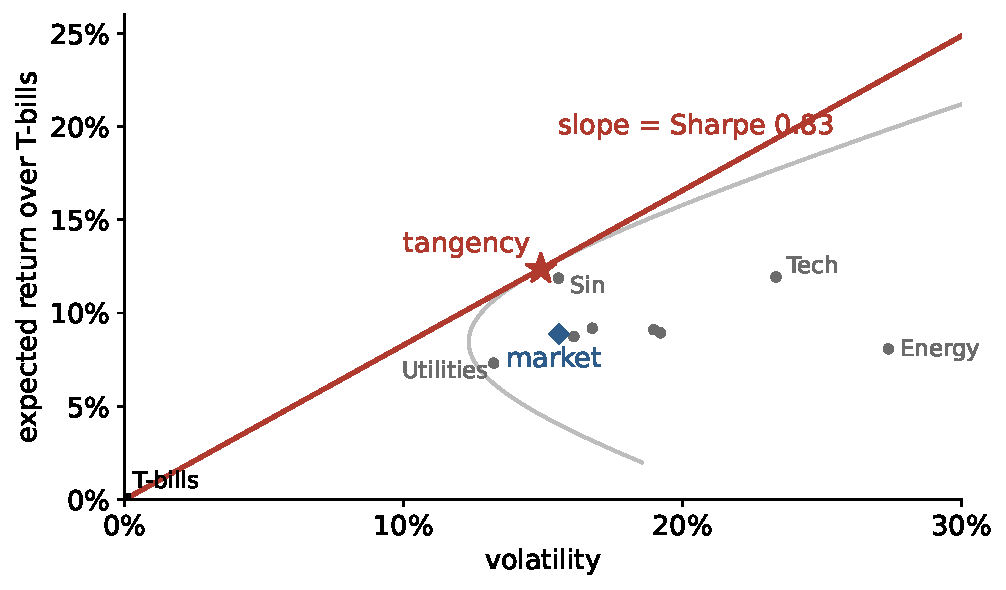
\includegraphics{figures/ca_frontier.pdf}}
\end{column}
\begin{column}{0.36\textwidth}
\begin{itemize}
\item Each dot is a sector, 1980--2026
\vskip 7pt
\item Mix the sectors and you can reach the curve
\vskip 7pt
\item Add T-bills, and you can reach any point on the straight line
\vskip 7pt
\item The steepest line wins. Its slope is the highest Sharpe ratio: \textcolor{red}{0.83}. The market: 0.57.
\end{itemize}
\end{column}
\end{columns}
\vskip 6pt
\centering Below the line, you could have earned more for the same risk.
\end{frame}

\begin{frame}{Two decisions, and they separate}
\begin{columns}[c]
\begin{column}{0.60\textwidth}
\adjustbox{max width=\textwidth, max height=0.68\textheight}{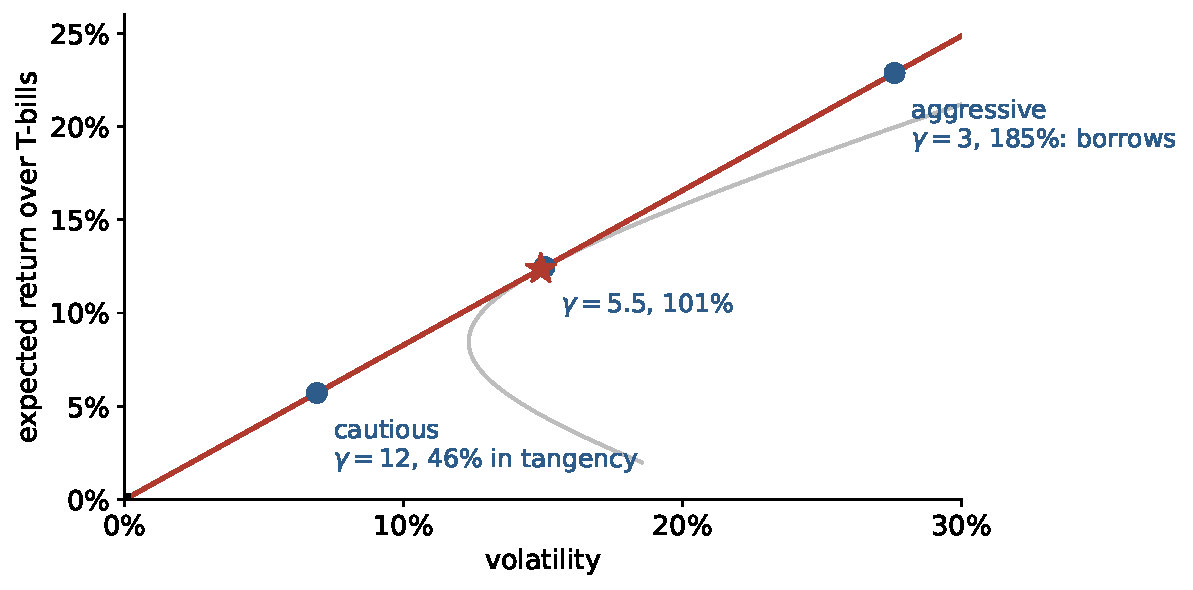
\includegraphics{figures/ca_frontier_people.pdf}}
\end{column}
\begin{column}{0.38\textwidth}
\textbf{1. How do you spread it?} \\[2pt]
The tangency portfolio. The same for everyone.
\vskip 12pt
\textbf{2. How much risk?} \\[2pt]
Where you sit on the line. Different for everyone.
\end{column}
\end{columns}
\vskip 8pt
\begin{beamercolorbox}[rounded=true,sep=7pt,center]{box1}
A cautious investor does not hold safer assets. They hold less of the same portfolio.
\end{beamercolorbox}
\end{frame}

\begin{frame}{That clean split rests on three assumptions}
\vskip 10pt
\begin{center}
\renewcommand{\arraystretch}{1.7}
\begin{tabular}{P{4.4cm}P{4.0cm}P{4.2cm}}
\toprule
the assumption & when it fails & what changes \\
\midrule
All your wealth is in financial markets & You have a job, a business, a house & Your portfolio should \textcolor{red}{tilt} \\
You choose for yourself & It is someone else's money & A mandate \textcolor{red}{bends the line} \\
You know $\mu$ and $\Sigma$ & You estimated them & \emph{Capital Allocation III} \\
\bottomrule
\end{tabular}
\end{center}
\vskip 14pt
\begin{center}
First the formula. Then we break the first two, with examples.
\end{center}
\end{frame}

\begin{frame}{One asset, no matrices}
You put a fraction $x$ of your money in one risky asset, the rest in T-bills.
\[ \max_{x}\;\; x\mu \;-\; \frac{\gamma}{2}\,x^{2}\sigma^{2} \]
{\small $\mu$: expected excess return \qquad $\sigma$: its volatility \qquad $\gamma$: how much you dislike variance}
\vskip 10pt
Differentiate and set to zero: $\;\mu - \gamma x\sigma^{2} = 0$
\vskip 12pt
\begin{beamercolorbox}[rounded=true,sep=8pt,center]{box1}
$\displaystyle x^{\star} \;=\; \frac{1}{\gamma}\,\frac{\mu}{\sigma^{2}}$
\end{beamercolorbox}
\vskip 12pt
\begin{itemize}
\item More return, hold more. More \emph{variance}, hold less, and it goes with the square.
\end{itemize}
\end{frame}

\begin{frame}{The volatility you run is your Sharpe ratio over your risk aversion}
Multiply both sides by $\sigma$: \qquad $\displaystyle x^{\star}\sigma \;=\; \frac{1}{\gamma}\,\frac{\mu}{\sigma} \;=\; \frac{SR}{\gamma}$
\vskip 10pt
\begin{center}
\renewcommand{\arraystretch}{1.3}
\begin{tabular}{cccl}
\toprule
$\gamma$ & weight in the market & volatility you run & \\
\midrule
1 & 3.66 & 57\% & nobody does this \\
2 & 1.83 & 29\% & \\
\textcolor{red}{5} & \textcolor{red}{0.73} & \textcolor{red}{11\%} & about three-quarters in stocks \\
10 & 0.37 & 6\% & \\
\bottomrule
\end{tabular}
\end{center}
{\small The market, 1980--2026: 8.9\% a year over T-bills, 15.6\% volatility, Sharpe ratio 0.57}
\vskip 8pt
\begin{itemize}
\item The formula answers the question you asked. It will recommend 3.7 times leverage if you hand it $\gamma=1$.
\end{itemize}
\end{frame}

\begin{frame}{Volatility management is this formula with $\sigma$ moving}
\[ x^{\star}_{t} \;=\; \frac{1}{\gamma}\,\frac{\mu_{t}}{\sigma_{t}^{2}} \]
\vskip 2pt
\begin{center}
\renewcommand{\arraystretch}{1.2}
\begin{tabular}{lccccc}
\toprule
UMD, by last month's volatility & calm & 2 & 3 & 4 & volatile \\
\midrule
average return (\% a year) & 10.7 & 12.4 & 6.8 & 7.2 & \textcolor{red}{$-0.3$} \\
volatility (\% a year) & 6.5 & 9.1 & 11.1 & 16.5 & \textcolor{red}{28.3} \\
\bottomrule
\end{tabular}
\end{center}
\vskip 8pt
\begin{itemize}
\item When volatility rises, the mean does not rise with it. So $\mu/\sigma^{2}$ falls, and you should hold less.
\vskip 6pt
\item Dividing by last month's variance was $x^{\star}$, with a guess that $\mu$ stays put. Same signal, same stocks: Sharpe ratio \textcolor{red}{0.45 $\rightarrow$ 0.94}.
\end{itemize}
\vskip 6pt
\hfill {\small We come back to this in \emph{Conditional Strategies}.}
\end{frame}

\begin{frame}[label=appendix_equiv_back]{Many assets: the same three steps}
Now $W$ and $\mu$ are vectors, and $\Sigma$ is the covariance matrix.
\[ \max_{W}\;\; W'\mu \;-\; \frac{\gamma}{2}\,W'\Sigma W
   \qquad\Longrightarrow\qquad \mu - \gamma\,\Sigma W = 0 \]
\vskip 6pt
\begin{beamercolorbox}[rounded=true,sep=8pt,center]{box1}
$\displaystyle W^{\star} \;=\; \frac{1}{\gamma}\,\Sigma^{-1}\mu$
\end{beamercolorbox}
\vskip 12pt
\begin{itemize}
\item The inverse is where the division used to be
\vskip 6pt
\item This is the mean-variance efficient portfolio, the tangency portfolio. It has the highest Sharpe ratio there is.
\vskip 6pt
\item It needs two things: $\mu$ and $\Sigma$. Remember that.
\end{itemize}
\vskip 4pt
\hfill \hyperlink{appendix_equiv}{\beamerbutton{Three ways to get here}}
\end{frame}

\begin{frame}{Two portfolios draw the whole curve}
\begin{columns}[c]
\begin{column}{0.60\textwidth}
\adjustbox{max width=\textwidth, max height=0.76\textheight}{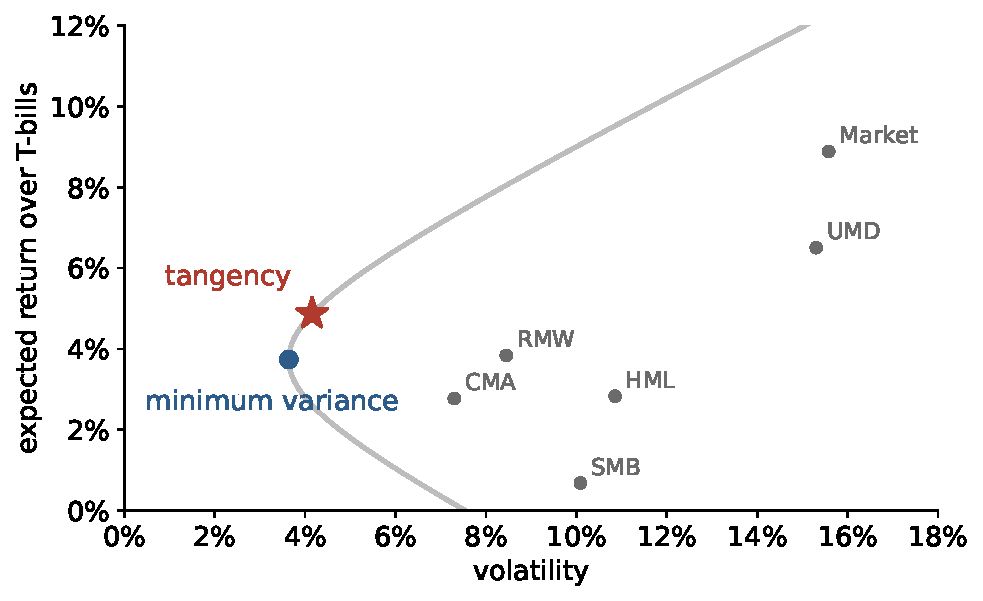
\includegraphics{figures/ca_fac_curve.pdf}}
\end{column}
\begin{column}{0.38\textwidth}
Six factors, 1980--2026. Each scaled so the weights add to one:
\vskip 6pt
\textcolor{red}{Tangency:} $\;\Sigma^{-1}\mu$ \\[2pt]
{\small highest Sharpe ratio, \textcolor{red}{1.17}}
\vskip 6pt
\textcolor{blue}{Minimum variance:} $\;\Sigma^{-1}\mathbf{1}$ \\[2pt]
{\small lowest risk, 3.6\%. It never looks at $\mu$.}
\vskip 10pt
\begin{itemize}
\item Every point on the curve is a mix of these two
\vskip 6pt
\item Both beat every factor by far: diversification
\end{itemize}
\end{column}
\end{columns}
\end{frame}

\begin{frame}{One portfolio, any size}
\begin{columns}[c]
\begin{column}{0.58\textwidth}
\adjustbox{max width=\textwidth, max height=0.74\textheight}{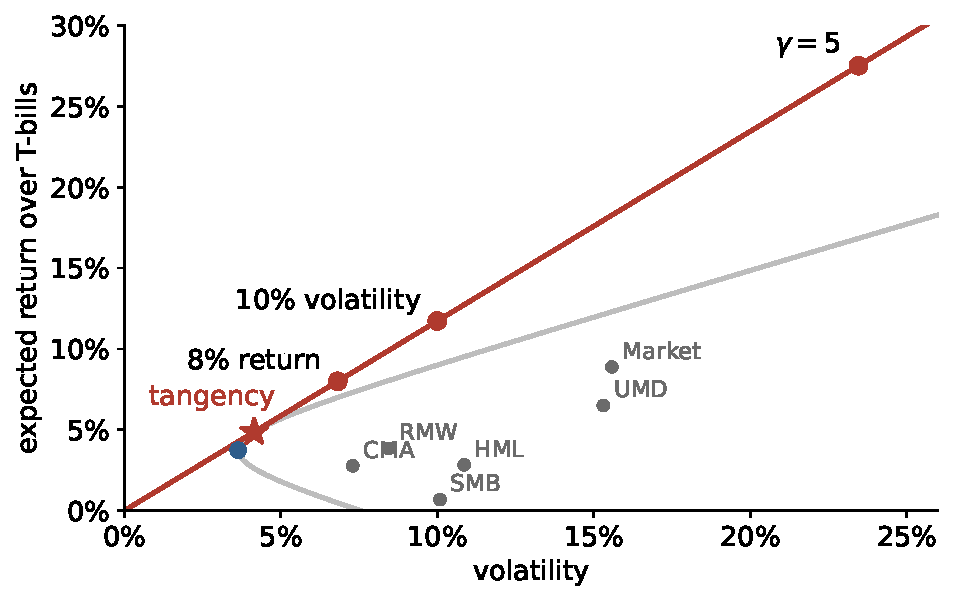
\includegraphics{figures/ca_fac_goals.pdf}}
\end{column}
\begin{column}{0.40\textwidth}
\renewcommand{\arraystretch}{1.25}
\adjustbox{max width=\textwidth}{\begin{tabular}{lcc}
\toprule
the goal & times tangency & vol \\
\midrule
8\% return & 1.6 & 6.8\% \\
10\% volatility & 2.4 & 10.0\% \\
$\gamma = 5$ & 5.6 & 23.5\% \\
$\gamma = 1$ & \textcolor{red}{28.2} & \textcolor{red}{117\%} \\
\bottomrule
\end{tabular}}
\vskip 10pt
\begin{itemize}
\item Same mix, same Sharpe ratio, 1.17. Only the size changes.
\vskip 6pt
\item $\gamma=1$ is off the chart. The formula answers the question you asked.
\end{itemize}
\end{column}
\end{columns}
\end{frame}

\begin{frame}{Does a new asset move the frontier?}
\begin{center}
\adjustbox{max width=\textwidth, max height=0.60\textheight}{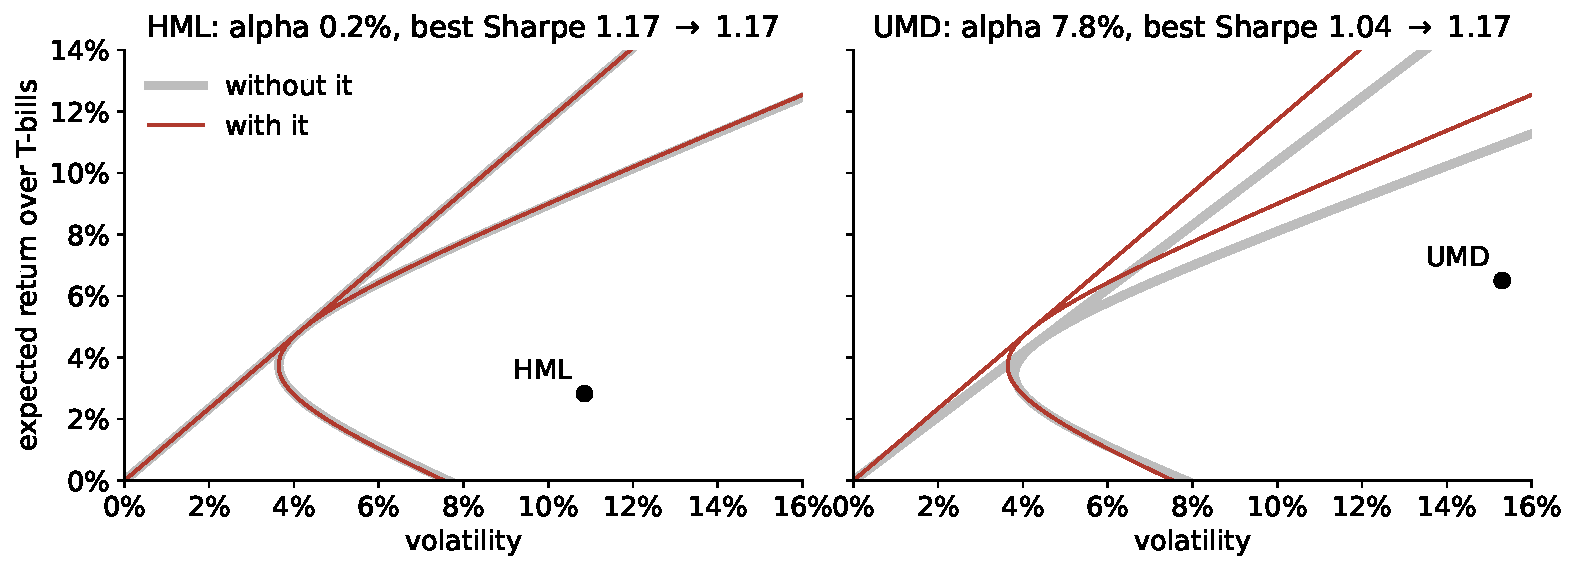
\includegraphics{figures/ca_fac_span.pdf}}
\end{center}
\begin{itemize}
\item HML has a Sharpe ratio of 0.26. Take it away and the frontier does not move.
\vskip 5pt
\item Momentum has 0.43, not so different. Take it away and the best Sharpe ratio falls by \textcolor{red}{0.13}.
\vskip 5pt
\item So a good Sharpe ratio on its own is not what moves the frontier. What is?
\end{itemize}
\end{frame}

\begin{frame}[label=span]{The alpha test is a test of the frontier}
Regress the new asset on the tangency portfolio of what you already hold:
\[ R_{\text{new}} = \textcolor{red}{\alpha} + \beta\, R_{\text{tangency}} + \varepsilon
\qquad\qquad SR^{2}_{\text{with}} = SR^{2}_{\text{without}} + \left(\frac{\textcolor{red}{\alpha}}{\sigma_{\varepsilon}}\right)^{2} \]
\vskip 2pt
\begin{center}
\renewcommand{\arraystretch}{1.1}
\adjustbox{max width=\textwidth}{\begin{tabular}{lccccc}
\toprule
add this factor to the other five & Sharpe alone & $\alpha$ a year & $t$ & best Sharpe without & with \\
\midrule
Market & 0.57 & 12.7\% & 6.1 & 0.74 & 1.17 \\
RMW & 0.45 & 4.1\% & 3.6 & 1.03 & 1.17 \\
\textcolor{red}{UMD} & 0.43 & \textcolor{red}{7.8\%} & \textcolor{red}{3.5} & \textcolor{red}{1.04} & \textcolor{red}{1.17} \\
CMA & 0.38 & 2.2\% & 2.8 & 1.09 & 1.17 \\
\textcolor{red}{HML} & 0.26 & \textcolor{red}{0.2\%} & \textcolor{red}{0.2} & \textcolor{red}{1.17} & \textcolor{red}{1.17} \\
SMB & 0.07 & 1.2\% & 0.9 & 1.17 & 1.17 \\
\bottomrule
\end{tabular}}
\end{center}
\vskip 4pt
\begin{beamercolorbox}[rounded=true,sep=6pt,center]{box1}
$\alpha = 0$ means the tangency portfolio already spans the new asset. You have run this test all semester.
\end{beamercolorbox}
\hfill \hyperlink{appendix_span}{\beamerbutton{Why the $\alpha$ is the same}}
\end{frame}

\begin{frame}{Now: the notebook}
\vskip 2pt
\begin{beamercolorbox}[rounded=true,sep=7pt,center]{box1}
\textbf{Notebook: Capital Allocation I} \ --- \ build the frontier, one step at a time
\end{beamercolorbox}
\vskip 10pt
\begin{enumerate}
\item \textbf{Tangency, then minimum variance.} Six factors, line by line.
\vskip 4pt
\item \textbf{Draw the frontier} from those two portfolios.
\vskip 4pt
\item \textbf{One portfolio, many goals.} $\gamma$, a return target, a volatility target, all on one picture.
\vskip 4pt
\item \textbf{Add a factor.} Run the alpha test on momentum, then on HML.
\end{enumerate}
\vskip 8pt
{\small \textbf{Bring back:} why does HML, with a positive Sharpe ratio, add nothing? Would you drop it? \\[2pt]
Stop at \textbf{Back to the slides}; the challenge after it is homework.}
\end{frame}

\begin{frame}{What the notebook showed}
\vskip 8pt
\begin{itemize}
\item \textbf{The mix and the size are separate.} Four goals, one tangency portfolio, one Sharpe ratio.
\vskip 10pt
\item \textbf{Assets earn their place through alpha.} HML: positive Sharpe ratio, no alpha, no effect. The other factors already span it.
\vskip 10pt
\item \textbf{That does not mean drop value forever.} Its alpha is $0.2\% \pm 1.2\%$, in this sample, gross of costs. \emph{Capital Allocation III} is about exactly this.
\end{itemize}
\vskip 14pt
\begin{beamercolorbox}[rounded=true,sep=7pt,center]{box1}
Everything so far assumed the same tangency portfolio is right for everyone. Is it?
\end{beamercolorbox}
\vskip 10pt
\centering {\small From here we go back to the sectors: tilts and mandates need things with names.}
\end{frame}

%================================================================== HOW MUCH RISK
\begin{frame}{How much risk? First: whose money is it?}
\vskip 10pt
\begin{columns}[t]
\begin{column}{0.47\textwidth}
\textbf{The principal}: your own money
\vskip 8pt
\begin{itemize}
\item How much do you mind losing?
\vskip 5pt
\item When do you need it?
\vskip 5pt
\item What are you saving for?
\vskip 5pt
\item \textcolor{red}{What else do you own?}
\end{itemize}
\end{column}
\begin{column}{0.47\textwidth}
\textbf{The delegate}: someone else's money
\vskip 8pt
\begin{itemize}
\item A volatility target
\vskip 5pt
\item A stop-loss, a point where you are fired
\vskip 5pt
\item A tracking-error budget
\vskip 5pt
\item Limits on what you can hold
\end{itemize}
\end{column}
\end{columns}
\vskip 20pt
\begin{center}
Both are answers to one question: where on the line?
\end{center}
\end{frame}

\begin{frame}{The principal: what is the worst you could stand?}
The market fell \textcolor{red}{50\%} from 2007 to 2009. If it happens again, how much could you stand to lose? \\ Nobody knows their $\gamma$. Everybody can answer this.
\vskip 10pt
\begin{center}
\renewcommand{\arraystretch}{1.35}
\begin{tabular}{cccc}
\toprule
the worst you could stand & so hold in the market & volatility you run & your $\gamma$ \\
\midrule
10\% & 20\% & 3\% & 18 \\
20\% & 40\% & 6\% & 9 \\
30\% & 60\% & 9\% & 6 \\
50\% & 100\% & 16\% & 3.7 \\
\bottomrule
\end{tabular}
\end{center}
\vskip 10pt
\begin{itemize}
\item Answer it before the fall. Selling at the bottom is the expensive way to learn your $\gamma$.
\vskip 6pt
\item Same market, four people: each row is a different point on the same line.
\end{itemize}
\end{frame}

\begin{frame}[label=back_stop]{The delegate: a stop-loss is a limit on volatility}
\begin{columns}[c]
\begin{column}{0.58\textwidth}
\adjustbox{max width=\textwidth, max height=0.72\textheight}{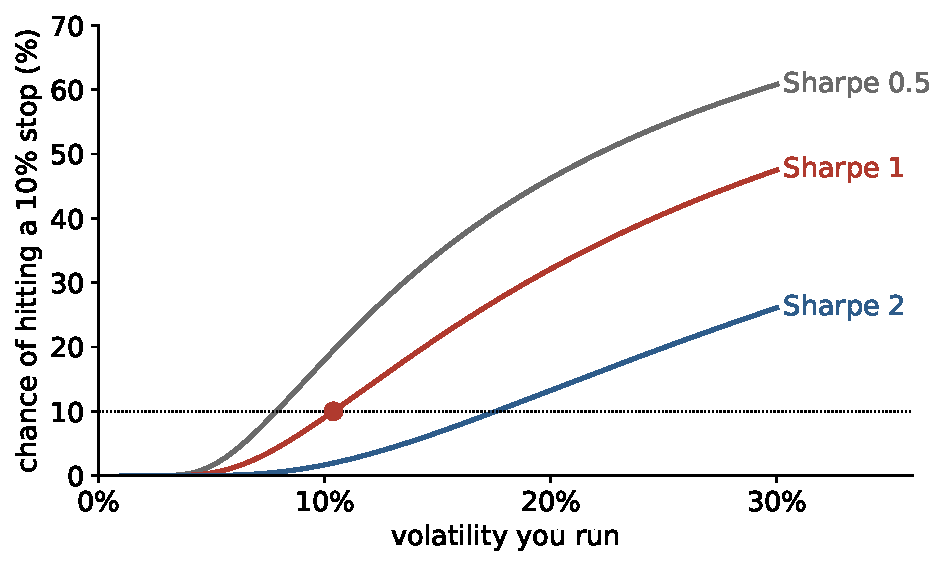
\includegraphics{figures/ca_stop.pdf}}
\end{column}
\begin{column}{0.40\textwidth}
\begin{itemize}
\item A pod shop might halve a team's capital after a 5\% loss, and close it at 7.5\%
\vskip 8pt
\item The stop is in percent, so volatility decides how often you hit it
\vskip 8pt
\item Sharpe 1, 10\% stop: at 10\% volatility, 9\% a year. At 20\% volatility, \textcolor{red}{32\%}.
\vskip 8pt
\item A better strategy can run more risk
\end{itemize}
\end{column}
\end{columns}
\vskip 4pt
\hfill \hyperlink{appendix_stop}{\beamerbutton{The formula}}
\end{frame}

\begin{frame}{A stop sets your place on the line}
\vskip 2pt
\begin{center}
\renewcommand{\arraystretch}{1.3}
\begin{tabular}{lcccc}
\toprule
your stop & 5\% & 7.5\% & 10\% & 20\% \\
\midrule
volatility for a 10\% chance of hitting it in a year, Sharpe 1 & 5\% & 8\% & 10\% & 21\% \\
the $\gamma$ that volatility implies, $SR/\sigma$ & \textcolor{red}{19} & 13 & 10 & 5 \\
\bottomrule
\end{tabular}
\end{center}
\vskip 8pt
\begin{itemize}
\item Rule of thumb, at Sharpe 1: run a volatility about equal to your stop
\vskip 6pt
\item The principal cannot give you their $\gamma$. A stop gives you one.
\vskip 6pt
\item Why they need it: a share of the gains and no share of the losses rewards volatility
\vskip 6pt
\item \emph{Hiring and Firing} fired on the appraisal ratio, which leverage cannot change. A stop in percent can be managed by running less risk. That is the point, and the cost.
\end{itemize}
\end{frame}

\begin{frame}{Your biggest asset is not in the market}
\vskip 4pt
\begin{center}
\renewcommand{\arraystretch}{1.35}
\begin{tabular}{lccc}
\toprule
 & financial wealth, $W$ & human capital, $H$ & $h = H/W$ \\
\midrule
at 22, starting at \$100k & \$10k & \textcolor{red}{\$2.3m} & 230 \\
at 45, earning \$150k & \$500k & \$2.2m & 4 \\
at 65, retiring & \$2m & \$0 & 0 \\
\bottomrule
\end{tabular}
\end{center}
{\small Human capital: wages to 62, growing 2\% a year, discounted at 5\%. Stylized.}
\vskip 10pt
\begin{itemize}
\item Human capital is an asset, and you cannot sell it
\vskip 6pt
\item It has a beta. It goes up and down with some things and not others.
\vskip 6pt
\item If it is most of your wealth, ignoring it means choosing most of your portfolio by accident
\end{itemize}
\end{frame}

\begin{frame}[label=back_hc]{Your job is a position}
Choose the financial account so that account plus job is the portfolio you want:
\vskip 10pt
\begin{beamercolorbox}[rounded=true,sep=8pt,center]{box1}
$\displaystyle w \;=\; \underbrace{(1+h)\,\frac{1}{\gamma}\Sigma^{-1}\mu}_{\text{the same tangency portfolio, sized for total wealth}} \;-\; \underbrace{h\,b}_{\text{short what looks like your job}}$
\end{beamercolorbox}
\vskip 8pt
{\small $h = H/W$ \qquad $b$: slopes from regressing your job's return on asset returns \qquad $\mu$, $\Sigma$: as before}
\vskip 10pt
\begin{itemize}
\item Your job already holds $b$. So the account holds less of it.
\vskip 6pt
\item With no job, $h=0$, and it is the formula from before
\vskip 6pt
\item Merton (1971), Bodie, Merton and Samuelson (1992)
\end{itemize}
\vskip 2pt
\hfill \hyperlink{appendix_hc}{\beamerbutton{Derivation}}
\end{frame}

\begin{frame}{A safe job: the same mix, more risk}
\begin{columns}[c]
\begin{column}{0.60\textwidth}
\adjustbox{max width=\textwidth, max height=0.74\textheight}{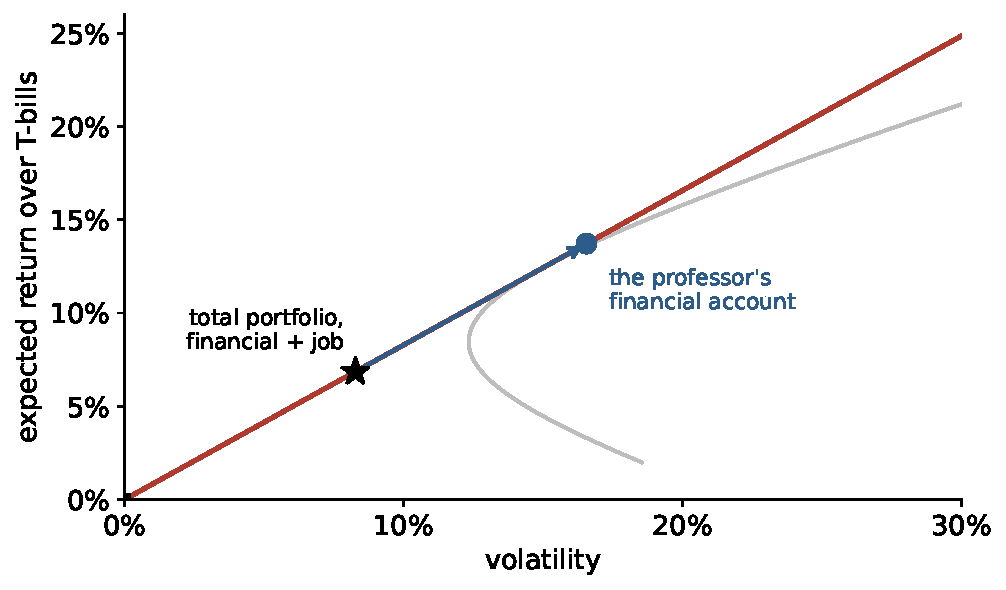
\includegraphics{figures/ca_hc_safe.pdf}}
\end{column}
\begin{column}{0.38\textwidth}
\begin{itemize}
\item A tenured professor: the job pays like a bond, $b = 0$
\vskip 8pt
\item They already own a lot of ``T-bills''. So the account takes the risk.
\vskip 8pt
\item Same mix, further along the line: here 17\% volatility, not 8\%
\vskip 8pt
\item The job runs out, $h$ falls, and the account moves back
\end{itemize}
\vskip 6pt
{\small $\gamma = 10$, $H = W$}
\end{column}
\end{columns}
\end{frame}

\begin{frame}{Now a job that is not safe}
\vskip 14pt
\begin{center}
{\large Same wealth, same risk aversion, same job security.\\[4pt] One is a software engineer: AI makes them more valuable.\\[4pt] One is a legal translator: AI may replace them.}
\vskip 18pt
Who should hold more tech stocks?
\vskip 18pt
\pollbox{blue}{\textbf{A}\ \ The engineer} \hfill
\pollbox{red}{\textbf{B}\ \ The translator} \hfill
\pollbox{gray}{\textbf{C}\ \ The same}
\end{center}
\end{frame}

\begin{frame}{AI: two accounts, one portfolio}
\begin{columns}[c]
\begin{column}{0.58\textwidth}
\adjustbox{max width=\textwidth, max height=0.72\textheight}{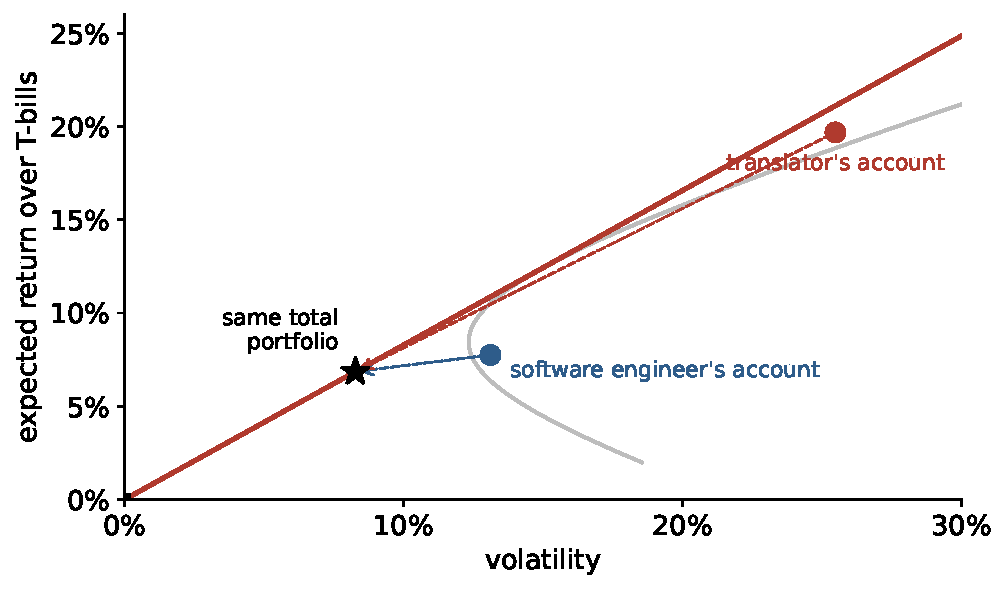
\includegraphics{figures/ca_hc_ai.pdf}}
\end{column}
\begin{column}{0.40\textwidth}
{\small $H = W$, $\gamma = 10$. Job's return: $\pm 0.5\times$ Tech.}
\vskip 6pt
\renewcommand{\arraystretch}{1.2}
\begin{tabular}{lc}
\toprule
 & Tech in account \\
\midrule
engineer & \textcolor{blue}{$-11\%$} \\
safe job & $+39\%$ \\
translator & \textcolor{red}{$+89\%$} \\
\bottomrule
\end{tabular}
\vskip 8pt
\begin{itemize}
\item The translator is buying insurance: AI wins, the job loses, the account pays
\vskip 5pt
\item Add the job back and both are at the star
\end{itemize}
\end{column}
\end{columns}
\end{frame}

\begin{frame}{Think it through: what does it move with, and which way do you tilt?}
\scriptsize
\renewcommand{\arraystretch}{1.28}
\begin{center}
\begin{tabular}{P{3.1cm}P{4.5cm}P{4.9cm}}
\toprule
who & what it moves with & the account \\
\midrule
tenured professor & nothing much, like a bond & same mix, more risk \\
investment banker & the market and Finance; the bonus falls with them & less Finance, less market \\
oil engineer in Houston & Energy, and so does the house & less Energy \\
software engineer & Tech, and AI & less Tech \\
translator, paralegal & against AI & more Tech \\
small-business owner & their sector, and one firm & less of that sector, less risk overall \\
homeowner & house prices in one city & less real estate \\
retiree & no job, $h = 0$ & the account is everything: less risk \\
pension fund & owes long-dated payments: a \emph{short} bond & holds long bonds, to hedge what it owes \\
\bottomrule
\end{tabular}
\end{center}
\normalsize
\vskip 4pt
\centering Now you: what will your job move with?
\end{frame}

\begin{frame}{All of them on one picture}
\begin{columns}[c]
\begin{column}{0.62\textwidth}
\adjustbox{max width=\textwidth, max height=0.76\textheight}{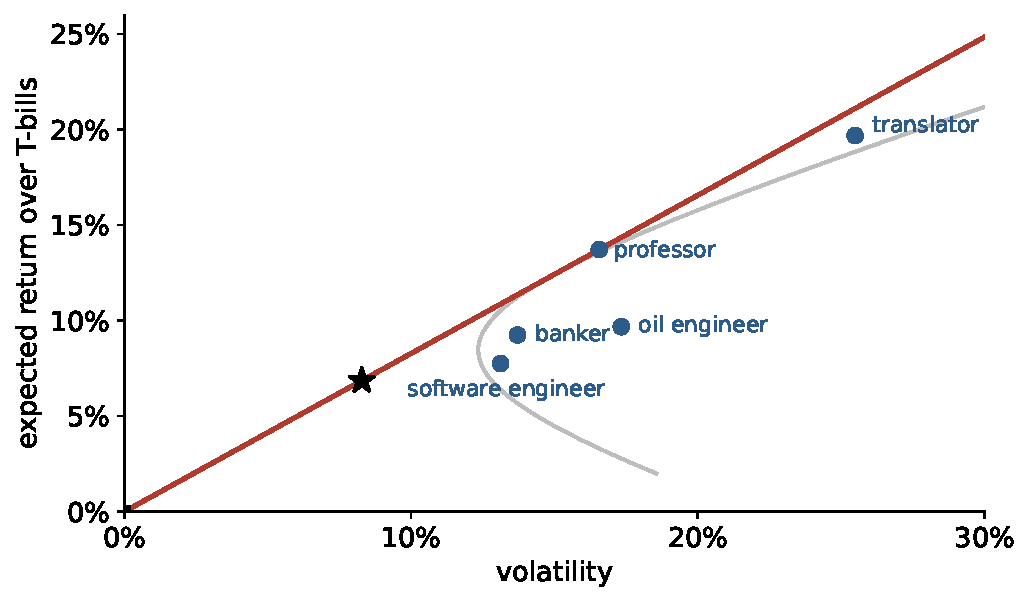
\includegraphics{figures/ca_hc_map.pdf}}
\end{column}
\begin{column}{0.36\textwidth}
\begin{itemize}
\item Same $\gamma$, same wealth, same star
\vskip 8pt
\item The safe job stays on the line. Every other account falls below it.
\vskip 8pt
\item Account Sharpe ratios: 0.59 to 0.77, against 0.83
\end{itemize}
\vskip 10pt
\begin{beamercolorbox}[rounded=true,sep=6pt,center]{box1}
Below the line, on purpose. Judge the account alone and it looks like a mistake.
\end{beamercolorbox}
\end{column}
\end{columns}
\end{frame}

\begin{frame}{What people actually do is the opposite}
\vskip 8pt
\begin{itemize}
\item \textbf{Enron, 2001.} About 60\% of its 401(k) assets were in Enron stock. When it failed, employees lost the job and the savings together.
\vskip 12pt
\item \textbf{Familiarity.} Investors tilt \emph{toward} stocks close to their own income, not away from them (Massa and Simonov 2006)
\vskip 12pt
\item \textbf{Back to the poll.} The instinct is to hold what you know, so the engineer holds Tech.
\end{itemize}
\vskip 18pt
\begin{beamercolorbox}[rounded=true,sep=7pt,center]{box1}
What you know best is often what you already own too much of
\end{beamercolorbox}
\end{frame}

\begin{frame}{The limits of this}
\vskip 8pt
\begin{itemize}
\item \textbf{You cannot borrow against your job.} At 22 the formula wants many times your savings in the market. You cannot borrow that, so this limit is the one that binds.
\vskip 10pt
\item \textbf{Nobody can estimate $b$.} Think sign and rough size, not decimals.
\vskip 10pt
\item \textbf{Tech is not AI.} Which stocks win from AI is itself a forecast, and insurance has a price: the translator's account earns a lower Sharpe ratio.
\vskip 10pt
\item \textbf{Most job risk cannot be hedged.} One firm, one boss. What you cannot trade is background risk, and it lowers how much market risk you want (Heaton and Lucas 2000).
\end{itemize}
\end{frame}

\begin{frame}{A mandate bends the line: no shorting, no borrowing}
\begin{columns}[c]
\begin{column}{0.60\textwidth}
\adjustbox{max width=\textwidth, max height=0.74\textheight}{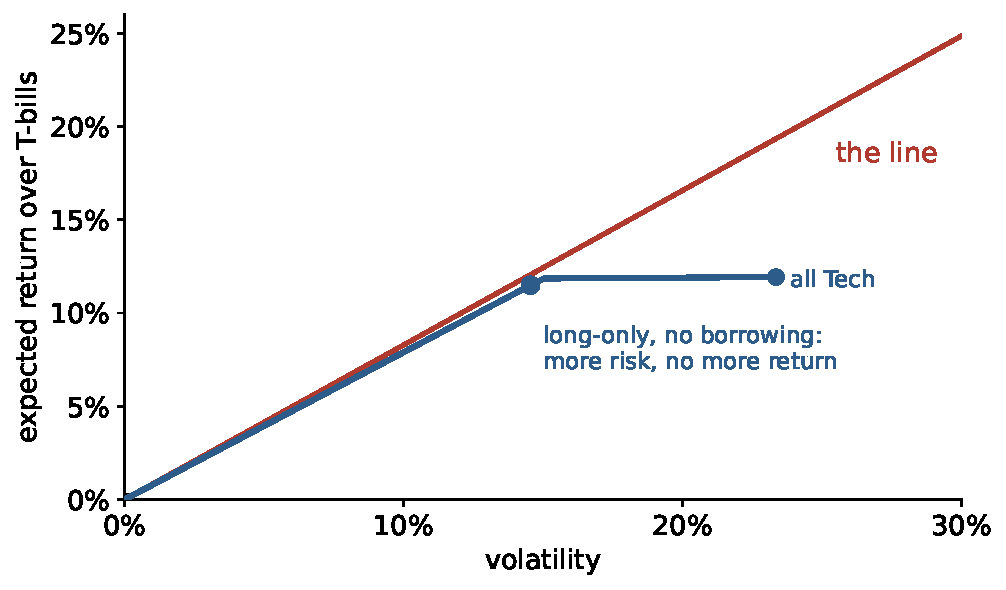
\includegraphics{figures/ca_mandate_longonly.pdf}}
\end{column}
\begin{column}{0.38\textwidth}
\begin{itemize}
\item No shorting barely costs here: 0.83 to 0.79
\vskip 8pt
\item No borrowing is what bites. At 18\% volatility: 11.9\%, not \textcolor{red}{14.9\%}.
\vskip 8pt
\item To take more risk you must hold riskier assets, not more of the tangency
\vskip 8pt
\item Many do, and that may be why high-beta assets earn too little (Black 1972; Frazzini and Pedersen 2014)
\end{itemize}
\end{column}
\end{columns}
\end{frame}

\begin{frame}{Exclusions and ESG: the price depends on what you exclude}
\begin{columns}[c]
\begin{column}{0.60\textwidth}
\adjustbox{max width=\textwidth, max height=0.74\textheight}{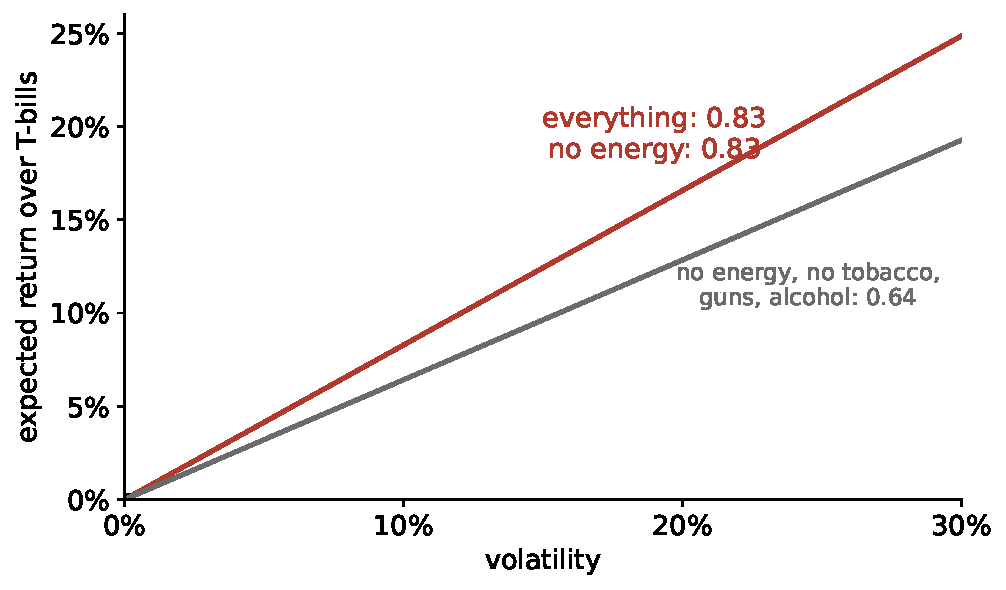
\includegraphics{figures/ca_mandate_esg.pdf}}
\end{column}
\begin{column}{0.38\textwidth}
\begin{itemize}
\item No energy: 0.83 to 0.83. It cost nothing here.
\vskip 8pt
\item No tobacco, guns, alcohol: 0.83 to \textcolor{red}{0.64}. The tangency was 94\% in them.
\vskip 8pt
\item Excluded stocks may earn more \emph{because} they are excluded (Hong and Kacperczyk 2009)
\vskip 8pt
\item Accepting a lower Sharpe ratio for what you value is a preference, not an error (Pedersen, Fitzgibbons and Pomorski 2021)
\end{itemize}
\end{column}
\end{columns}
\end{frame}

\begin{frame}{Factor limits: zero beta takes one leg off the triangle}
\begin{columns}[c]
\begin{column}{0.60\textwidth}
\adjustbox{max width=\textwidth, max height=0.74\textheight}{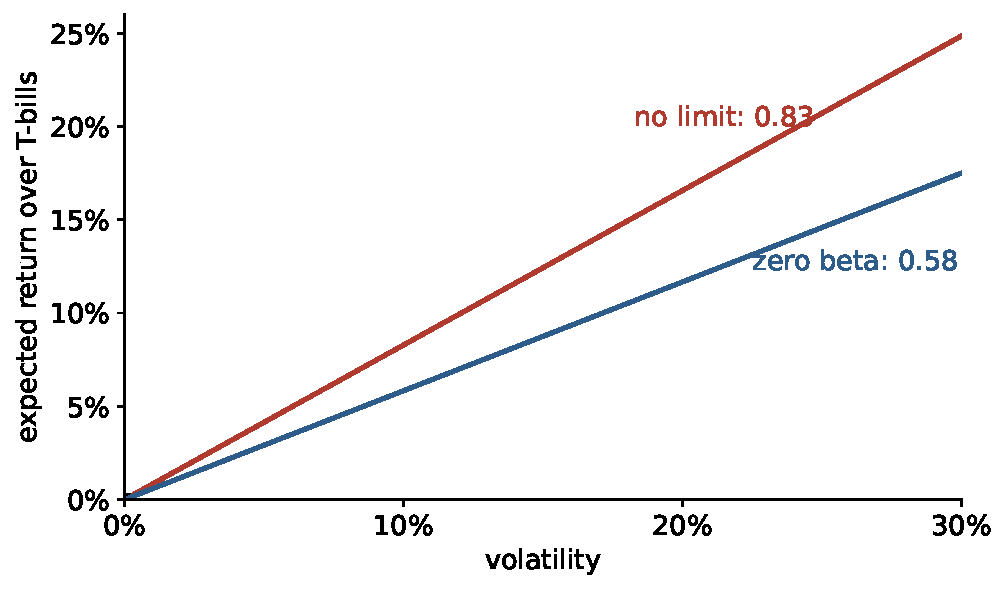
\includegraphics{figures/ca_mandate_beta.pdf}}
\end{column}
\begin{column}{0.38\textwidth}
\begin{itemize}
\item Market-neutral: the best you can do with no market exposure is \textcolor{red}{0.58}
\vskip 8pt
\item Why accept it? The principal already owns the market. They pay you for what they do not have.
\vskip 8pt
\item Limits on size, value or momentum work the same way: each removes something the optimizer wanted
\vskip 8pt
\item The hedged book is next class
\end{itemize}
\end{column}
\end{columns}
\end{frame}

\begin{frame}{Tracking error: a budget around a benchmark}
\begin{columns}[c]
\begin{column}{0.60\textwidth}
\adjustbox{max width=\textwidth, max height=0.74\textheight}{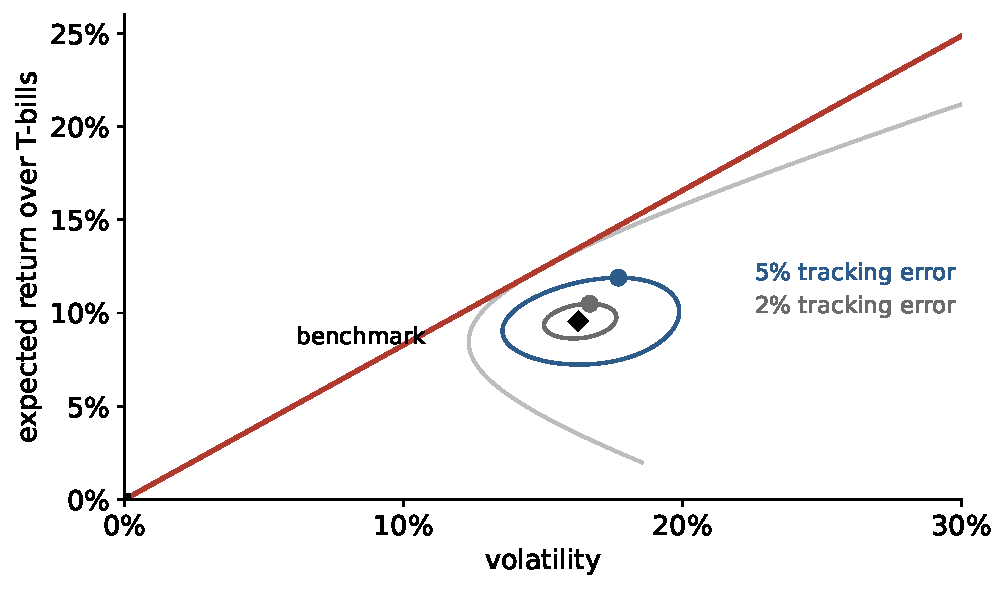
\includegraphics{figures/ca_mandate_te.pdf}}
\end{column}
\begin{column}{0.38\textwidth}
\begin{itemize}
\item You are judged on the gap to the benchmark, so your budget is a small circle around it
\vskip 8pt
\item The best point on it is still below the line: Sharpe 0.63 at 2\%, 0.67 at 5\%
\vskip 8pt
\item Reaching the line at the benchmark's risk takes about \textcolor{red}{12\%} tracking error
\vskip 8pt
\item It also runs more total risk than the benchmark (Roll 1992). The manager does not count that; the owner does.
\end{itemize}
\end{column}
\end{columns}
\end{frame}

\begin{frame}{Every mandate has a price: the slope you lose}
\begin{columns}[c]
\begin{column}{0.60\textwidth}
\adjustbox{max width=\textwidth, max height=0.70\textheight}{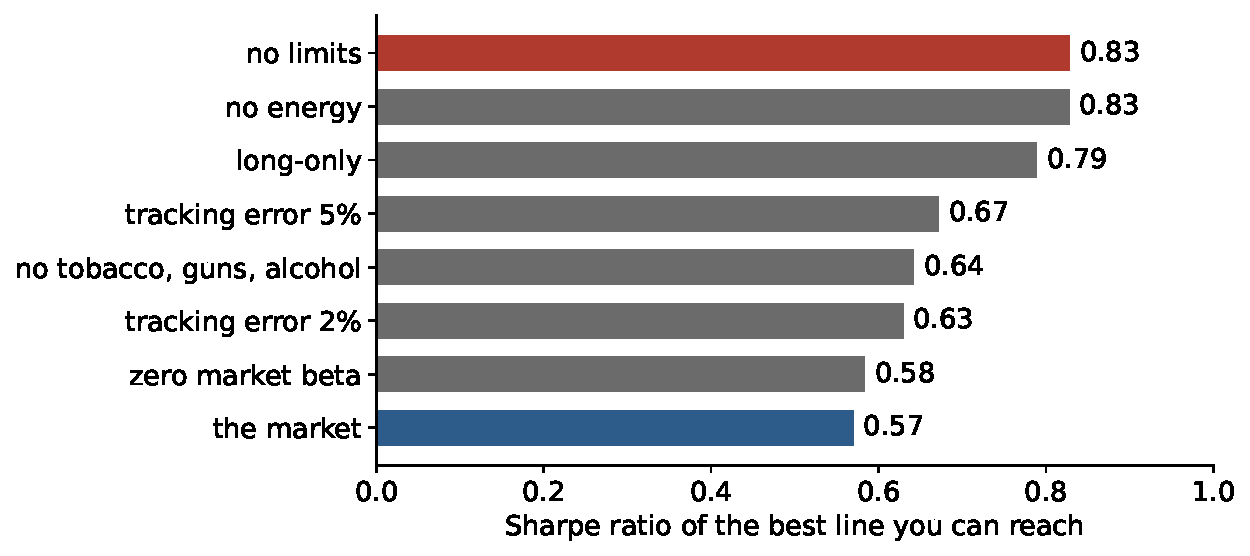
\includegraphics{figures/ca_mandate_price.pdf}}
\end{column}
\begin{column}{0.38\textwidth}
\begin{itemize}
\item Measure the price first, then decide whether it is worth paying
\vskip 8pt
\item A mandate can be worth it: the owner has other holdings, values, and limited trust
\vskip 8pt
\item All of this is in sample, and tobacco did very well. In \emph{Capital Allocation III} a constraint can even \emph{help}, because the inputs are estimated.
\end{itemize}
\end{column}
\end{columns}
\end{frame}

\begin{frame}{Takeaways}
\begin{enumerate}
\item Everyone wants the steepest line. How much risk is a separate decision, if all your wealth is financial.
\vskip 6pt
\item The volatility you run is your Sharpe ratio over your risk aversion. For a delegate, a stop sets it.
\vskip 6pt
\item Your job is a position. Hold the same tangency portfolio, minus what looks like your job.
\vskip 6pt
\item Every mandate has a price: the slope you lose. Measure it, then decide.
\end{enumerate}
\vskip 14pt
\begin{beamercolorbox}[rounded=true,sep=7pt]{box1}
\textbf{Homework: goals and mandates.} On the 49 industries: hit a volatility goal, a return goal and a leverage limit. Then take out more and more of the sin industries. What does it cost, and what would happen to their prices if everyone did it?
\end{beamercolorbox}
\end{frame}

%================================================================== APPENDIX
\appendix
\begin{frame}
\begin{center}
{\Large Appendix}
\end{center}
\end{frame}

\begin{frame}[label=appendix_span]{Why the alpha is the same both ways}
Take $W = \Sigma^{-1}\mu$. Its variance equals its mean: $W'\Sigma W = W'\mu = \mu'\Sigma^{-1}\mu$. Let $c$ be the covariances of the new asset with the old ones.
\vskip 8pt
\begin{itemize}
\item \textbf{On the tangency portfolio:} $\beta = c'W / W'\Sigma W$, so $\alpha = \mu_{\text{new}} - \beta\, W'\mu = \mu_{\text{new}} - c'\Sigma^{-1}\mu$
\vskip 6pt
\item \textbf{On all the assets:} $b = \Sigma^{-1}c$, so $\alpha = \mu_{\text{new}} - b'\mu = \mu_{\text{new}} - c'\Sigma^{-1}\mu$
\vskip 6pt
\item The same $\alpha$. The standard deviation is not the same: in the Sharpe formula, $\sigma_{\varepsilon}$ is the residual on \emph{all} the assets, which hedges more than the tangency portfolio alone.
\vskip 6pt
\item In the table, momentum's $\alpha$ is 7.84\% both ways. Scaling $W$ changes $\beta$, not $\alpha$.
\end{itemize}
\vskip 4pt
\hfill \hyperlink{span}{\beamerreturnbutton{Back}}
\end{frame}

\begin{frame}[label=appendix_equiv]{A: Three problems, one portfolio}
\renewcommand{\arraystretch}{1.7}
\begin{center}
\begin{tabular}{lll}
\toprule
maximize utility & $\max_{W}\; W'\mu - \frac{\gamma}{2}W'\Sigma W$ & $W = \frac{1}{\gamma}\Sigma^{-1}\mu$ \\
hit a return with the least variance & $\min_{W}\; W'\Sigma W$ s.t. $W'\mu = \bar\mu$ & $W = \frac{\bar\mu}{\mu'\Sigma^{-1}\mu}\Sigma^{-1}\mu$ \\
take a risk budget, earn the most & $\max_{W}\; W'\mu$ s.t. $W'\Sigma W = \bar\sigma^{2}$ & $W = \frac{\bar\sigma}{\sqrt{\mu'\Sigma^{-1}\mu}}\Sigma^{-1}\mu$ \\
\bottomrule
\end{tabular}
\end{center}
\vskip 10pt
\begin{itemize}
\item All three are a number times $\Sigma^{-1}\mu$. Only the size changes.
\vskip 6pt
\item The Sharpe ratio is the same in all three: $\sqrt{\mu'\Sigma^{-1}\mu}$.
\vskip 6pt
\item A delegate with a volatility target solves the third, and never needs $\gamma$.
\end{itemize}
\hfill \hyperlink{appendix_equiv_back}{\beamerreturnbutton{Back}}
\end{frame}

\begin{frame}[label=appendix_stop]{A: The chance of hitting a stop}
Treat the account as earning $\mu = SR\,\sigma$ a year with volatility $\sigma$, watched continuously. The chance of being down $D$ from the start at some point within $T$ years:
\[ P \;=\; \Phi\!\left(\frac{-D-\mu T}{\sigma\sqrt{T}}\right) \;+\; e^{-2\mu D/\sigma^{2}}\;\Phi\!\left(\frac{-D+\mu T}{\sigma\sqrt{T}}\right) \]
\vskip 6pt
\begin{itemize}
\item This counts losses from the start of the year. A stop on the drawdown from the peak is hit more often.
\vskip 6pt
\item Returns are assumed normal, and volatility constant. Real crashes jump through a stop.
\vskip 6pt
\item Monthly checks instead of continuous ones would lower the chance a little
\end{itemize}
\hfill \hyperlink{back_stop}{\beamerreturnbutton{Back}}
\end{frame}

\begin{frame}[label=appendix_hc]{A: Why your job is a position}
Per dollar of total wealth, you hold $x$ in the assets and $\phi = H/(W+H)$ in your job, whose return is $r_{H}$:
\[ \max_{x}\;\; x'\mu + \phi\,\mu_{H} - \frac{\gamma}{2}\Big(x'\Sigma x + 2\phi\, x'\sigma_{H} + \phi^{2}\sigma_{H}^{2}\Big) \quad\Rightarrow\quad x = \frac{1}{\gamma}\Sigma^{-1}\mu - \phi\,\Sigma^{-1}\sigma_{H} \]
{\small $\sigma_{H}$: the covariances between your job and the assets. $b = \Sigma^{-1}\sigma_{H}$ are the slopes from regressing $r_{H}$ on asset returns.}
\vskip 8pt
Per dollar of the account, $w = x\,(W+H)/W$, so with $h = H/W$:
\[ w \;=\; (1+h)\,\frac{1}{\gamma}\Sigma^{-1}\mu \;-\; h\,b \]
\begin{itemize}
\item With a job of $\pm 0.5\times$ Tech, $b$ is $\pm 0.5$ in Tech and zero elsewhere. Add the job back: $\frac{W}{W+H}\,w + \phi\,b = x^{\star}$, the star.
\vskip 4pt
\item The job is valued as if it can be priced like the assets it moves with
\end{itemize}
\hfill \hyperlink{back_hc}{\beamerreturnbutton{Back}}
\end{frame}

\begin{frame}{A: Data, and what to be careful about}
\begin{itemize}
\item \textbf{Six factors.} Ken French, 1980--2026, excess returns. They are long-short, so ``weights add to one'' only sets a scale.
\vskip 8pt
\item \textbf{Eight sectors.} Ken French's 49 industries, grouped by us, equal-weighted within a sector, over T-bills, 1980--2026. ``Other'' is left out. ``Sin'' is Smoke, Guns and Beer. The benchmark is the sector mix that best tracks the market.
\vskip 8pt
\item \textbf{In sample.} The frontier uses the same data it is judged on. Its 94\% in Sin is what happened, not a recommendation.
\vskip 8pt
\item \textbf{Human capital.} Every number is stylized: the job's beta on one sector is an assumption, chosen to make the tilt easy to see.
\vskip 8pt
\item \textbf{No costs, no capital limits.} Everything here is gross.
\end{itemize}
\end{frame}


\end{document}
